\documentclass[../main.tex]{subfiles}

\begin{document}

\subsection{Schelling's Dynamic Models Of Segregation - Overview}
Racial segregation has always been a major social problem in the world and especially in the US. Despite all efforts, racial and economical segregation is still around us. But why is it so hard to eradicate segregation?

In 1971, in the \textit{Journal of Mathematical Sociology}, the American economist \textit{Thomas C. Schelling} published a paper on \textit{Dynamic Models of Segregation}. He designed a simple agents-based model in order to explain why segregation is such a hard problem to combat. He showed that even if individuals (or agents) did not mind living in a mixed neighbourhood, they would still choose to move/segregate over time. Schelling did not use a very sophisticated model, but the output of his study was surprising: although individuals had no explicit desire to self-segregate, they would still do so. The model focuses on residential segregation of ethnic groups. It is a \textit{two-type agent model}. That is, the agents are of two types: white or black. This is the only characteristic that distinguishes the agents. In any other aspect, the agents are identical.

\subsection{How does the model work?}
Now, we are going to explain the two main models that Schelling used. We are going to start with the Spatial Proximity Model and then have a brief overview of the Bounded-Neighborhood Model. For the Spatial Proximity Model, Shelling starts by putting the population in a simple model (the linear model). Next, he organises the people in a  two-dimensional area. The general idea is displayed in the linear model as well as in the two-dimensions model. In this project we are focusing on the linear model since we are interested in automatically testing this model, using a computational multi-agent model.

\subsubsection{Spatial Proximity Models}
 In this model, everybody defines their neighbourhood by reference to his own position. An individual who is \textit{unhappy} with his neighbourhood, \textit{i.e.} he is not content with the mixture of his neighbourhood, would try to find a place, and move to that place, where his demands are satisfied. Hence, for each agent what matters is the colour ratio in his own neighbourhood. Schelling looks at what distributions of tolerance among individuals may result in a stable mixture. He looks at how different initial conditions and dynamics of the movement will impact the outcome and if there are any numerical constraints that could alter the results.

For these models, we are going to use two types of agents to help us represent these models: \z\ - representing a white individual and \x\ - representing a black individual.\\

\textbf{Linear Distribution} \\
The first spatial model, is a model where agents distribute themselves along a \textit{line}. Let us take for example a random distribution of 12 \z s and 12 \x s:

\begin{table}[H]
\begin{center}
\resizebox{\textwidth}{!}{\begin{tabular}{| c |c| c| c| c |c| c |c| c |c |c |c |c |c |c |c |c |c |c |c |c|c |c |c |c|}
\hline
\x & \x & \x & \z & \x & \z & \x &\z &\z &\z &\z & \x &\x &\z &\x &
\z &\z &\z &\x &\x &\z &\z &\x & \x \\
 \hline
\end{tabular}}
\end{center}
\caption*{Random Linear distribution - 12 whites and 12 blacks} 
\end{table}

Shelling interprets this reasonably random distribution as people spread in a line, each concerned with the colours of the people in their neighbourhood. Assume that each individual defines his neighbourhood as himself and the two individuals at his right and two individuals at his left. One of the assumptions that Schelling makes regarding the satisfaction of an individual in his neighbourhood is that half of the neighbours of the individual to be the same colour as himself. \textit{e.g.} In our case, with a neighbourhood of 4 people (excluding himself), an individual would be content if at least 2 people are the same colour as himself. In special cases, like when the individual is at the end of the line, the two neighbours on the side towards the central plus maybe one outboard neighbour would represent the local neighbourhood and hence at least half (one out of two neighbours or two out of three neighbours) must be the same colour.

Looking at our random distribution, we can see that, according to the above rule, for a neighbourhood of size two (4 people in total), 10 out of the 24 agents are unhappy (unhappy agents are on positions: 4, 7, 12, 14, 15,19, 20, 21, 22, 23). Here, we put a dot over the unhappy agents.

\begin{table}[H]
\begin{center}
\resizebox{\textwidth}{!}{\begin{tabular}{| c |c| c| c| c |c| c |c| c |c |c |c |c |c |c |c |c |c |c |c |c|c |c |c |c|}
\hline
 & & & $\cdot$ & &  & $\cdot$ & & & & & $\cdot$ & &$\cdot$ &$\cdot$ & &
 & &$\cdot$ &$\cdot$ &$\cdot$ &$\cdot$ &$\cdot$ &  \\
 1 &2 & 3&4 &5 & 6 & 7 &8 &9 &10 &11 &12 &13 &14 &15 &16 &17
 &18 &19 &20 &21 &22 &23 &24  \\
\x & \x & \x & \z & \x & \z & \x &\z &\z &\z &\z & \x &\x &\z &\x &
\z &\z &\z &\x &\x &\z &\z &\x & \x \\
 \hline
\end{tabular}}
\end{center}
\caption*{The dot represents a discontent agent} 
\end{table}

The next step was to define a rule about how the individuals can move. A discontent person moves to the nearest position where he would be satisfied (at least half of his neighbours are like oneself). Hence, he is looking at passing the minimum number of individuals and intrudes himself between two others when he gets to a place where he is happy (satisfied). The order in which they move is set alternating turns from left to right. \textit{i.e.} the first person to move would be the \z\ on position 4 followed by \x\ on position 23 and so on. Once they start moving, we notice that some people who were discontented become content while other which initially were content will become discontent. The rule is that if an initial unhappy individual becomes happy by the time his turn comes, he will not move. After going through all the initial unsatisfied individuals, any other individuals that became unhappy due to the movement of the previous agents, they will have their turn to move.

After one step, the distribution looks as follows. Agent 4 moves to position 6.
\begin{table}[H]
\begin{center}
\resizebox{\textwidth}{!}{\begin{tabular}{| c |c| c| c| c |c| c |c| c |c |c |c |c |c |c |c |c |c |c |c |c|c |c |c |c|}
\hline
 & & &  &$\cdot$ &  & $\cdot$ & & & & & $\cdot$ & &$\cdot$ &$\cdot$ & &
 & &$\cdot$ &$\cdot$ &$\cdot$ &$\cdot$ &$\cdot$ &  \\
 1 &2 & 3&5 &6 & 4 & 7 &8 &9 &10 &11 &12 &13 &14 &15 &16 &17
 &18 &19 &20 &21 &22 &23 &24  \\
\x & \x & \x & \x & \z & \z & \x &\z &\z &\z &\z & \x &\x &\z &\x &
\z &\z &\z &\x &\x &\z &\z &\x & \x \\
 \hline
\end{tabular}}
\end{center}
\end{table}

Notice that Agent 6 that was initially content is now discontent. The next to move is Agent 23. The nearest position for Agent 23 is swapping place with Agent 24. This makes Agent 24 discontent.
\begin{table}[H]
\begin{center}
\resizebox{\textwidth}{!}{\begin{tabular}{| c |c| c| c| c |c| c |c| c |c |c |c |c |c |c |c |c |c |c |c |c|c |c |c |c|}
\hline
 & & &  &$\cdot$ &  & $\cdot$ & & & & & $\cdot$ & &$\cdot$ &$\cdot$ & &
 & &$\cdot$ &$\cdot$ &$\cdot$ &$\cdot$ &$\cdot$ &  \\
 1 &2 & 3&5 &6 & 4 & 7 &8 &9 &10 &11 &12 &13 &14 &15 &16 &17
 &18 &19 &20 &21 &22 &24 &23  \\
\x & \x & \x & \x & \z & \z & \x &\z &\z &\z &\z & \x &\x &\z &\x &
\z &\z &\z &\x &\x &\z &\z &\x & \x \\
 \hline
\end{tabular}}
\end{center}
\end{table}

Next to move is Agent 7. Notice we skipped Agent 6 since he was not discontent to begin with.

\begin{table}[H]
\begin{center}
\resizebox{\textwidth}{!}{\begin{tabular}{| c |c| c| c| c |c| c |c| c |c |c |c |c |c |c |c |c |c |c |c |c|c |c |c |c|}
\hline
 & & &  & &  &  & & & & & $\cdot$ & &$\cdot$ &$\cdot$ & &
 & &$\cdot$ &$\cdot$ &$\cdot$ &$\cdot$ &$\cdot$ &  \\
 1 &2 & 3&5 &7 & 6 & 4 &8 &9 &10 &11 &12 &13 &14 &15 &16 &17
 &18 &19 &20 &21 &22 &24 &23  \\
\x & \x & \x & \x & \x & \z & \z &\z &\z &\z &\z & \x &\x &\z &\x &
\z &\z &\z &\x &\x &\z &\z &\x & \x \\
 \hline
\end{tabular}}
\end{center}
\end{table}

The discontent agents continue to move according to Schelling's turn function rules, until we reach the following final configuration.
\begin{table}[H]
\begin{center}
\resizebox{\textwidth}{!}{\begin{tabular}{| c |c| c| c| c |c| c |c| c |c |c |c |c |c |c |c |c |c |c |c |c|c |c |c |c|}
\hline
 1 &2 & 3&5 &7 & 6 & 4 &8 &9 &10 &11 &13 &12 &15 &14 &16 &17
 &18&22&21 &19 &20 &24 &23  \\
\x &\x & \x & \x & \x & \z & \z &\z &\z &\z &\z & \x & \x &  \x &
\z &\z &\z &\z &\z &\z &\x &\x & \x &\x \\
 \hline
\end{tabular}}
\end{center}
\end{table}

The result is five clusters of like individuals where every agent is content.\\

\textbf{Area Distribution}\\
Looking into two dimensions space, having a relative position is not something that we could implement easily. In the linear model, when an agent was discontent, he was moving from a position in between two individuals to a position between two other individuals, \textit{i.e.} relative position. 

For the Area Distribution, Schelling divides the space into rectangle spaces, each agent occupies one rectangle space. Hence, in the model there are going to be rectangle spaces occupied by agents, be them black (\x) or white (\z), or they will be \textit{vacant}. An agent, is able to move only to a vacant square and when he moves he leaves a place vacant. Similar to the linear model, he would move only if he is "unhappy" in his neighbourhood. Hence, the model's basic assumption is that an individual located in the middle of the neighbourhood that has less than \verb|p| percent individuals like himself, will try to relocate to a neighbourhood for which this percentage is met. The percent, \verb|p|, for which the agents are satisfied is a predefined tolerance threshold. The higher this percentage is, the \textit{less tolerant} the agent is.

Let us now look at one of Schelling's random distribution model (Table 1). There is an equal number of whites (\z)\ and blacks (\x)\ and 70 vacant places. There are 25 \x\ and 18 \z\ that are discontent (have neighbours less than half of like colour). We also can check that \z s on average have 53\% neighbours of the same colour and \x s have 46\%.


\begin{table}[H]
\begin{center}
\resizebox{\textwidth}{!}{\begin{tabular}{| c |c| c| c| c |c| c |c| c |c |c |c |c |c |c |c|}
\hline
\z & \x & \x & \x & \x & \z & \z & \z & \z &    &    & \x & \x &    & \z & \z  \\
\hline
\z &    & \x & \z & \z & \z &    & \x & \x &    &    & \x &    & \x & \z &     \\
\hline
\x &    & \x & \z & \z & \x & \x &    & \x &    &    & \z & \x &    & \x & \x  \\
\hline
\x &    &    & \x & \x &    &    & \z & \x & \x & \x & \z & \z &    &    &     \\
\hline
\z &    & \z & \z & \x & \x & \x & \x &    &    & \x &    & \x &    & \z & \z  \\
\hline
   & \x & \z & \x &    & \z & \z & \x &    &    & \z & \z &    &    & \x & \x  \\
\hline
\x & \z & \z & \x &    &    &    &    & \z & \z & \z & \x & \x & \x &    &     \\
\hline
\z &    & \x & \z &    & \x & \x &    & \x & \z & \z & \z &    &    &    & \x  \\
\hline
\z &    & \x & \z &    &    &    &    & \x & \x & \z &    &    &    &    & \x  \\
\hline
\z & \z &    &    &    & \x &    &    & \z & \x & \z & \z & \z & \z & \x & \x  \\
\hline
   & \z & \x & \x & \z & \z & \z & \z &    & \z & \x & \x &    & \z & \x & \x  \\
\hline
\x &    & \z & \x & \z & \x &    & \z & \z & \x & \z & \x & \z &    & \z &     \\
\hline
   & \z & \z &    &    & \z & \x & \z & \x & \z & \z & \z &    &    & \x & \x  \\
\hline
\end{tabular}}
\end{center}
\caption{Initial condition of one of Schelling's experiments} 
\end{table}

In most of Schelling's examples, the neighbourhood of any agent \textbf{\textcolor{purple}{A}} is defined as the 8 surrounding square. See \textit{Table 2}.

\begin{table}[H]
\begin{center}
\begin{tabular}{| c |c| c|}
\hline
\textbf{\textcolor{mygreen}{N}} & \textbf{\textcolor{mygreen}{N}} & \textbf{\textcolor{mygreen}{N}} \\
\hline
\textbf{\textcolor{mygreen}{N}} & \textbf{\textcolor{purple}{A}} & \textbf{\textcolor{mygreen}{N}}  \\
\hline
\textbf{\textcolor{mygreen}{N}} & \textbf{\textcolor{mygreen}{N}} & \textbf{\textcolor{mygreen}{N}}  \\
\hline
\end{tabular}
\end{center}
\caption{Neighbourhood} 
\end{table}

As in the linear model, a demand and a moving rule must be established. For this example, we have the same demand as previously seen: no fewer than half of one's neighbours be of the same colour. Also, the individuals who are discontent will move to the nearest vacant place that satisfies their demands. However, it is more complicated than in the linear model to define a rule to specify the order in which they move.

Starting at the upper-left corner going downwards and to the right, an equilibrum is achive as shown in Table 3. 

\begin{table}[H]
\begin{center}
\resizebox{\textwidth}{!}{\begin{tabular}{| c |c| c| c| c |c| c |c| c |c |c |c |c |c |c |c|}
\hline
\x & \x & \x & \x & \x &    &    &    &    & \x & \x & \x & \x &    & \z & \z  \\
\hline
\x & \x & \x & \x & \x & \x & \x & \x & \x & \x & \x & \x &    & \x & \z & \z  \\
\hline
\x & \x & \x & \x & \x & \x & \x & \x & \x & \x & \x &    & \x & \x & \z & \z  \\
\hline
\x &    &    & \x & \x & \x & \x & \x & \x & \x & \x &    &    & \x & \z & \z  \\
\hline
\z & \z & \z & \z & \x & \x & \x & \x & \x & \x & \x &    & \x &    &    &     \\
\hline
   & \z & \z & \z & \z & \z & \x & \x & \x & \z & \z &    & \x &    & \x & \x  \\
\hline
   & \z & \z & \z & \z & \z & \z & \z & \z & \z & \z & \z & \x & \x &    &     \\
\hline
\z &    &    & \z &    & \z & \z & \z &    & \z & \z & \z &    &    &    & \x  \\
\hline
\z &    &    & \z &    &    &    &    &    &    & \z &    &    &    &    & \x  \\
\hline
\z & \z &    &    &    &    &    &    & \z &    & \z & \z & \z &    & \x & \x  \\
\hline
   & \z &    &    & \z & \z & \z & \z &    & \z &    &    & \z & \z & \x & \x  \\
\hline
   &    & \z &    & \z &    &    & \z & \z &    & \z &    & \z & \z &    &     \\
\hline
   & \z & \z &    &    & \z &    & \z &    & \z & \z & \z &    &    & \x & \x  \\
\hline
\end{tabular}}
\end{center}
\caption{Stable segregation - moving left-to-right, up-down} 
\end{table}

Moving from centre outwards, the following equilibrium is achieved (Table 4):

\begin{table}[H]
\begin{center}
\resizebox{\textwidth}{!}{\begin{tabular}{| c |c| c| c| c |c| c |c| c |c |c |c |c |c |c |c|}
\hline
   & \x & \x & \x &    & \z & \z & \z &    &    &    & \x & \x &    & \z & \z  \\
\hline
   &    & \x & \x &    & \z & \z &    & \x &    &    & \x &    & \x & \z & \z  \\
\hline
\x &    & \x &    &    & \x & \x & \x & \x & \x & \x & \x &    & \x &    &     \\
\hline
\x & \x &    & \x & \x & \x &    &    & \x & \x & \x & \z & \z &    & \x & \x  \\
\hline
   & \z & \z & \x & \x & \x & \x & \x &    &    & \z & \z & \z &    &    &     \\
\hline
\z & \z & \z & \z & \x &    &    & \x & \z & \z & \z & \z & \x & \x & \x & \x  \\
\hline
\z & \z & \z & \z & \z &    & \x &    & \z & \z & \z &    & \x & \x &    &     \\
\hline
\z &    &    & \z & \z &    & \x &    & \z & \z & \z & \z &    &    &    & \x  \\
\hline
\z & \z & \x & \x &    &    &    & \x & \x & \z & \z & \z &    &    &    & \x  \\
\hline
\z & \z & \x & \x & \x & \x &    &    & \x & \x & \z & \z & \z & \z & \x & \x  \\
\hline
   & \z & \x & \x & \x & \z & \z & \z &    & \x & \x &    &    & \z & \x & \x  \\
\hline
   &    & \z &    & \z & \z &    & \z & \z & \x & \x & \x & \z & \z &    & \x  \\
\hline
   & \z & \z &    &    & \z &    & \z & \z & \z &    &    &    & \z &    & \x  \\
\hline
\end{tabular}}
\end{center}
\caption{Stable segregation - moving from centre outwards} 
\end{table}

Although, the process started from the same initial random distribution, two fairly different stable states were achieved. While in \textit{Table 3} the segregation is obvious (we could even talk about a complete segregation), in \textit{Table 4} it is not so clear that the segregation happened. Hence, the outcome of the movement depends a lot to which order the individuals move. However, all Schelling is trying to show in the paper is that segregation is still happening, the outcome is always a stable segregation, regardless of the movement rules.


\subsubsection{Bounded-Neighbourhood Model}
Although a lot less popular than the spatial proximity model, bounded - neighbourhood model  looks at a more realistic situation. It looks at neighbourhoods that have a limited capacity, like a school that can take a limited number of pupils or an office that has a certain number of employees.

Individuals do not define anymore their neighbourhood relatively to their location, but instead, there is a common definition of the neighbourhood (\verb|i.e.| a school) and its boundaries. The individual is either inside or outside the neighbourhood.

Another significant change in this model is that each person has their own tolerance, instead of an identical tolerance. \verb|i.e.| an individual might not be interested at all in the colour ratio in the neighbourhood that he is part of, while another(be he black or white) might only tolerate people of same colour like oneself. So the tolerance of each individual is defined as a straight line cumulative distribution plotted against the ration that the individual is willing to accept in the neighbourhood.

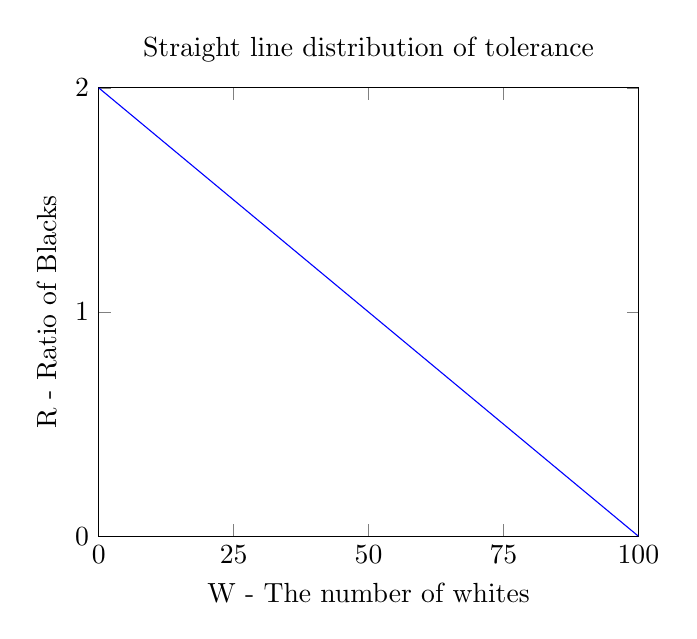
\begin{tikzpicture}
\begin{axis}[
    title={Straight line distribution of tolerance},
    xlabel={W - The number of whites},
    ylabel={R - Ratio of Blacks},
    xmin=0, xmax=100,
    ymin=0, ymax=2,
    xtick={0,25,50,75,100},
    ytick={0,1,2},
]
 
\addplot[
    color=blue,
    ]
    coordinates {
    (100,0)(0,2)
    };
\end{axis}
\end{tikzpicture}

The above graph, represents the tolerance distribution of whites. The most tolerant white person can accept a black-white ratio of 2 to 1, while the least tolerant white person cannot stand the presence of any black people.


In order to study the dynamics in this system, Schelling makes the assumption that people both leave and return. People in the neighbourhood move out if a certain ratio is not met and people outside the neighbourhood move in if they see that their requirements are met. We notice that even if people are permitted to return to the area, they might never do so since their requirements might never be met. \verb|e.g.| If an individual moved out because the cost of living in that location were high, by moving back to the same area the costs will probably still be the same.

Another assumption that is made is that everybody knows the ratio colour at the moment they make a choice. When it comes to moving rules, the assumption is that between two dissatisfied people of same colour, the one that is least tolerant moves out first. When it comes to moving in, the most tolerant one moves in first.

The straight line tolerance schedule can be translated into a parabolic curve as shown below. 

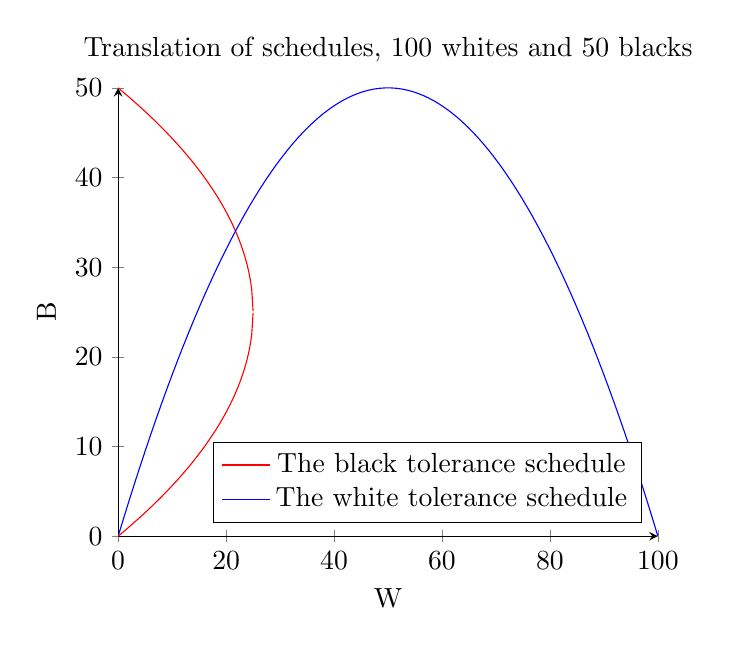
\begin{tikzpicture}
\begin{axis}[
    title={Translation of schedules, 100 whites and 50 blacks},
    axis lines = left,
    xlabel = {W},
    ylabel = {B},
    legend pos = south east,
]
%Below the red parabola is defined
\addplot [
    domain= 0:25, 
    samples=100, 
    color=red,
]
{sqrt(-25*x + 625) + 25};
\addlegendentry{The black tolerance schedule}

%Here the blue parabloa is defined
\addplot [
    domain=0:100, 
    samples=100, 
    color=blue,
    ]
    {(-1) * x^2 /50 + 2*x};
\addlegendentry{The white tolerance schedule}
\addplot [
    domain= 0:25, 
    samples=100, 
    color=red,
]
{-1*sqrt(-25*x + 625) + 25};
\end{axis}
\end{tikzpicture}

In the above example, the number of blacks is half the number of whites. In the intersection of the white tolerance schedule and the black tolerance schedule, we have a good mixture of blacks and whites such that everybody is content. However, if we are under the white tolerance schedule curve, but not under the blacks curve, we are in a situation where all whites are content, but not all the blacks. Similarly for the blacks.

Another example Schelling presents, is having the same number of blacks and whites (100 each). This is represented below. 

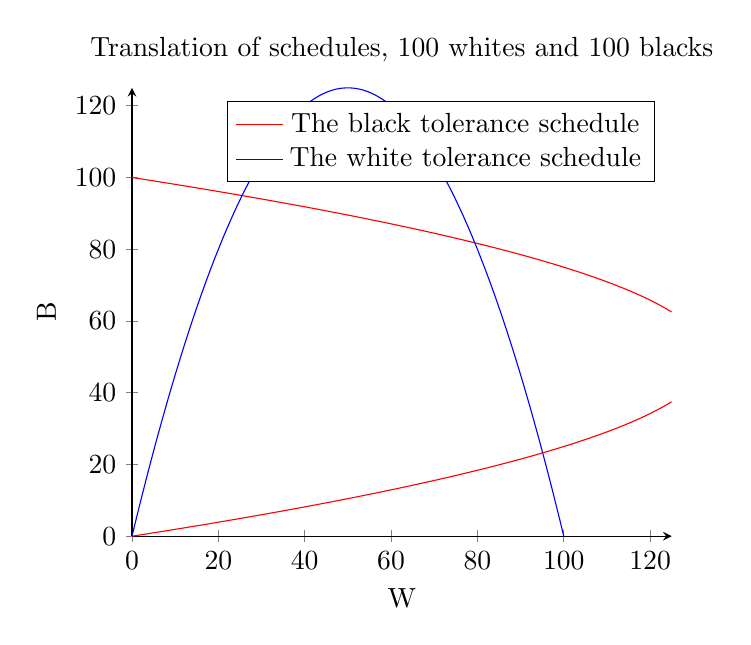
\begin{tikzpicture}
\begin{axis}[
    title={Translation of schedules, 100 whites and 100 blacks},
    axis lines = left,
    xlabel = {W},
    ylabel = {B},
    legend pos = north east,
]
%Below the red parabola is defined
\addplot [
    domain= 0:125, 
    samples=100, 
    color=red,
]
{1/2 *  sqrt(-75*x + 10000) + 50};
\addlegendentry{The black tolerance schedule}

%Here the blue parabola is defined
\addplot [
    domain=0:100, 
    samples=100, 
    color=blue,
    ]
    {(-1) * x^2 /20 + 5*x};
\addlegendentry{The white tolerance schedule}
\addplot [
    domain= 0:125, 
    samples=100, 
    color=red,
]
{-1/2 *  sqrt(-75*x + 10000) + 50};
\end{axis}
\end{tikzpicture}

These graphs allow us to interpret how the population changes within the area, the dynamics motion. For example, in the above graph, if we are located above the blacks tolerance curve, but below the white tolerance curve then we are in a situation where blacks are entering and whites are leaving because they are not content. On the right of the whites curve, below the blacks curve, we have whites coming in while blacks departing. 

The area that is under both parabolas is a stable area. However, Schelling claims that at some point or another this "temporary stable equilibrium" will be disturbed since people who are in the neighbourhood will not leave, while people from outside the neighbourhood who would be content inside the area, will enter the neighbourhood. It is a matter of which colour is going to dominate, whether we are going up or right in our graph. 

Hence, Schelling makes a very important statement and that is: "There are only two stable equilibria. One consists of all the blacks and no whites, the other all the whites and no blacks."

\subsubsection{Tipping Model}
In the final model, Schelling presents a combination of the two earlier models. By altering the entering rules, he tries to reproduce a phenomena that he says that was closely observed by \textit{A.J.Mayer (1960)}\cite[]{mayer}, the "tipping phenomenon". Schelling claims that if a large enough minority group enters a neighbourhood, this will lead to "tipping", that is causing the initial residents to evacuate the area and we would end up with a neighbourhood with a majority of the opposite colour (or any characteristic we consider) than the initial one.
 




\end{document}